%%%%%%%%%%%%%%%%%%%%%%%%%%%%%%%%%%%%%%%%%%%%%%%%%%%%%%%%%%%%%%%%%%%%%%%%
%    INSTITUTE OF PHYSICS PUBLISHING                                   %
%                                                                      %
%   `Preparing an article for publication in an Institute of Physics   %
%    Publishing journal using LaTeX'                                   %
%                                                                      %
%    LaTeX source code `ioplau2e.tex' used to generate `author         %
%    guidelines', the documentation explaining and demonstrating use   %
%    of the Institute of Physics Publishing LaTeX preprint files       %
%    `iopart.cls, iopart12.clo and iopart10.clo'.                      %
%                                                                      %
%    `ioplau2e.tex' itself uses LaTeX with `iopart.cls'                %
%                                                                      %
%%%%%%%%%%%%%%%%%%%%%%%%%%%%%%%%%%
%
%
% First we have a character check
%
% ! exclamation mark    " double quote  
% # hash                ` opening quote (grave)
% & ampersand           ' closing quote (acute)
% $ dollar              % percent       
% ( open parenthesis    ) close paren.  
% - hyphen              = equals sign
% | vertical bar        ~ tilde         
% @ at sign             _ underscore
% { open curly brace    } close curly   
% [ open square         ] close square bracket
% + plus sign           ; semi-colon    
% * asterisk            : colon
% < open angle bracket  > close angle   
% , comma               . full stop
% ? question mark       / forward slash 
% \ backslash           ^ circumflex
%
% ABCDEFGHIJKLMNOPQRSTUVWXYZ 
% abcdefghijklmnopqrstuvwxyz 
% 1234567890
%
%%%%%%%%%%%%%%%%%%%%%%%%%%%%%%%%%%%%%%%%%%%%%%%%%%%%%%%%%%%%%%%%%%%
%
\documentclass[12pt]{iopart}
\newcommand{\gguide}{{\it Preparing graphics for IOP Publishing journals}}
%Uncomment next line if AMS fonts required
%\usepackage{iopams}  
\usepackage{graphicx}
\begin{document}

\title[]{Absolute calibration of gravitational wave detector using gravity field and photon pressure}

\author{Yuki Inoue, Sadakazu Haino, Nobuyuki Kanda, Yujiro Ogawa, Toshikazu Suzuki, Takayuki Tomaru, Takahiro Yamamoto, Takaaki Yokozawa}

\address{IOP Publishing, Temple Circus, Temple Way, Bristol BS1 6HG, UK}
\ead{iyuki@post.kek.jp}
\vspace{10pt}
\begin{indented}
\item[]June 2018
\end{indented}

\begin{abstract}
\end{abstract}

%
% Uncomment for keywords
%\vspace{2pc}
%\noindent{\it Keywords}: XXXXXX, YYYYYYYY, ZZZZZZZZZ
%
% Uncomment for Submitted to journal title message
%\submitto{\JPA}
%
% Uncomment if a separate title page is required
%\maketitle
% 
% For two-column output uncomment the next line and choose [10pt] rather than [12pt] in the \documentclass declaration
%\ioptwocol
%



\section{Introduction}

%Overview of GW observation
The discovery of the gravitational wave give us the new probe for observing our universe. 
Instruments for measuring the gravitational wave must be designed for accuracy as well as precession.
The typical strain sensitivity of 2nd generation interferometric detectors(IFO), such as Advanced LIGO, Advanced Virgo, and KAGRA, are around $10^{-23}/\sqrt{Hz}$. In order to estimate the parameters of gravitational waves, such as masses, spins, redshift and distance, understanding of the systematic and statistical noise sources are critical.

%Calibration
To reduce the systematic errors of the gravitational wave calibration and reconstruction, we need to calibrate the response of IFO. The first generation of the photon calibrator is developed by the Grasgow. LIGO and Virgo employ the second generation photon calibrator for the calibration of time-dependent optical gain of IFO.  The frequency range of photon calibrator is between 10 and 3000Hz.  However, it has a challenging issue of the absolute calibration due to the accuracy of the absolute laser power of laser standard between each country. Therefore, current uncertainty of absolute power is a few percent.

%KAGRA and Our approach
The dynamic gravity field generator is one of the candidates to be able to solve the uncertainty problem of absolute calibration. Related techniques using photon calibrator and gravity field calibrator are described as Karuki. et. al and Matone et al.
%Chap1 is XXXXX, … .

\section{Photon calibrator}
Photon calibrator (Pcal) relies on the photon radiation pressure from the power modulated laser beams reflecting on the test mass to apply periodic force via the recoil of photons. 
LIGO, Virgo and KAGRA employ the photon calibrator for the calibration of the interferometer response. The displacement of the test mass can be described as
\begin{equation}
 x = \frac{P \cos{\theta}}{2c} s(\omega)\left(1+\frac{M}{I}\vec{a} \cdot \vec{b} \right) , \label{pcal}
\end{equation}
where $P$ is absolute laser power, $\theta$ is incident angle of the Pcal laser, $M$ is mass of test mass, $\omega$ is angular frequency, $I$ is inertia, $\vec{a}$ and $\vec{b}$ are position vector of Pcal laser beams. $s(\omega)$ is transfer function between force and displacements. The laser power is stabilized less then design sensitivity. The stabilized laser is mounted on the transmitter module. The power is monitored by the average response of the photo detectors at the transmitter module and receiver module.  The uncertainty of displacement corresponds to uncertainty of laser power. 
The largest uncertainty of photon calibrator is uncertainty of laser power.
LIGO and KAGRA use the working standard to cross-calibrate the relative response of each interferometer. The uncertainty of  each  calibrator is 0.51 \%. For the absolute calibration, it is compared with the NIST laser power standard. We send Gold standard to NIST and calibrate the response of detector. After that, we bring the gold standard to LHO and calibrate the working standard Hanford, Livingston and KAGRA. The uncertainty of laser standard of each institute of standard is a few percent. 
The second largest uncertainty of photon calibrator is optical efficiency of optical path. the estimated uncertainty of optical efficiency in LIGO is 0.37 \%. We need to estimate the laser power response through the response of photo detector at the outside of vacuum chamber. 
The reduction of these uncertainties are essential for the gravitational wave observation.

\begin{figure}
\begin{center}
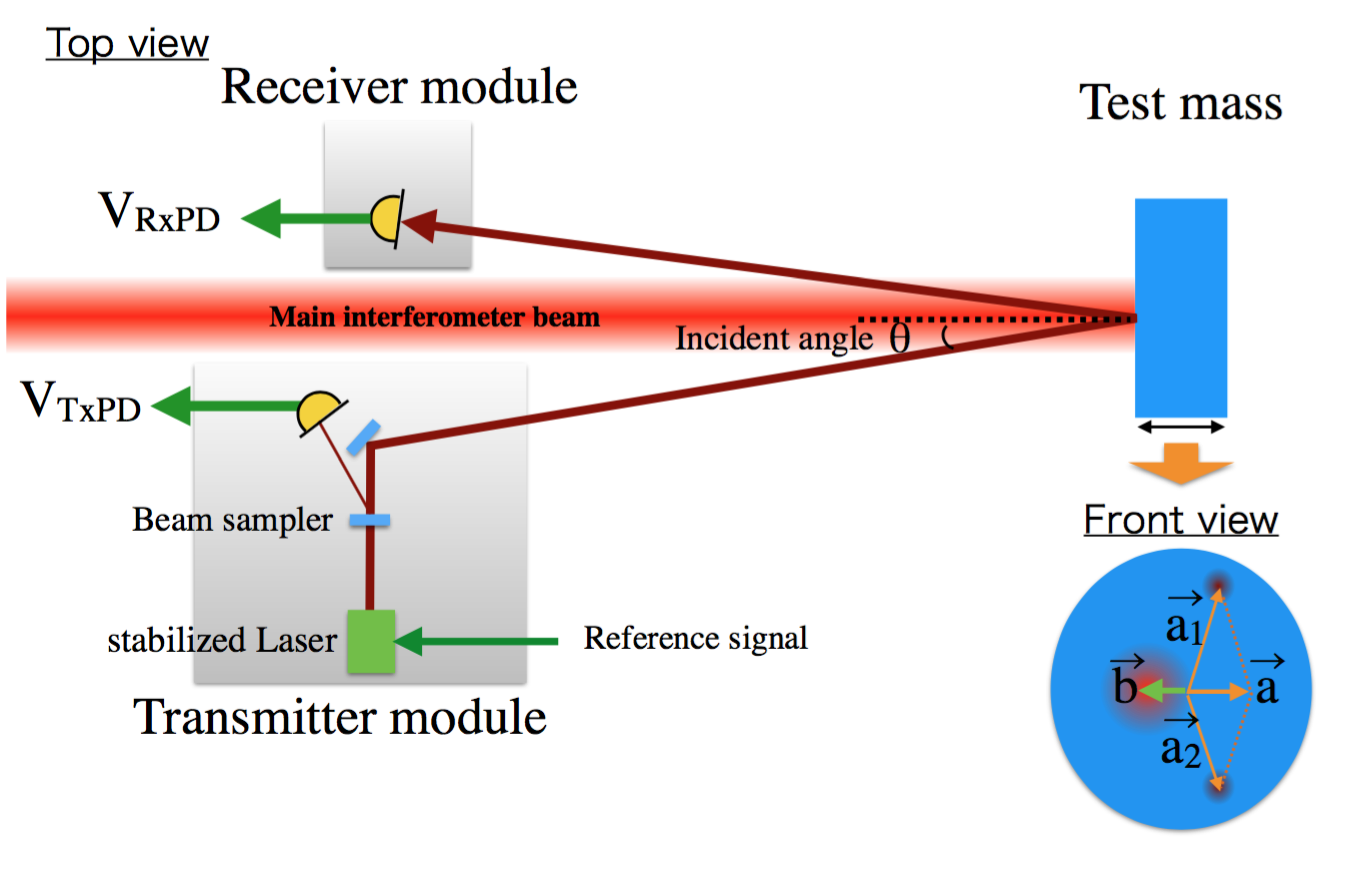
\includegraphics[width=12cm]{Pcal.eps}
\caption{Schematic view of photon calibrator. We place the stabilized laser on the transmitter module. The injected signal at the test masses is monitored by using the average of photo detector power between the transmitter module, $V_{TxPD}$ and  receiver module, $V_{RxPD}$.  The geometrical factor is characterized by the position vector of the main beam, $\vec{a}=\vec{a_1}+\vec{a_2}$, and photon calibrator beams, $\vec{b}$.}
\label{fig:Pcal}
\end{center}
\end{figure}

\begin{table}
\begin{center}
\caption{Specification summary of LIGO, Virgo and KAGRA photon calibrator\label{pcal}}
\footnotesize
\begin{tabular}{cccc}
\br
& KAGRA& advanced LIGO& advanced Virgo \\
\mr
Mirror material & Sapphire & Silica & Silica \\
 Mirror mass & 22.8 kg & 40 kg & 40 kg \\
  Mirror diameter & 220 mm & 340 mm & 350 mm \\
    Mirror thickness & 150 mm & 200 mm & 200 mm \\
 Distance of Pcal from ETM & 36 m & 8 m & 1.5 m \\
  Pcal laser power & 20 W & 2W & 3 W \\
  Laser frequency & 1047 nm & 1047 nm &1047 nm\\
  Incident angle& 0.72 deg & 8.75 deg &30 deg \\
\br
\end{tabular}
\end{center}
\end{table}

\section{Gravity field calibrator}
To solve the calibration uncertainty, we propose the gravity field calibrator. The original idea is described in Matone. et.al. The gravity field calibrator generate the gravity field at the end of test mass. By rotating the multipole masses, the rotor placed in the vacuum chamber for isolating the acoustic noise. To monitor the frequency, we mount the 10-bit encoder. We monitor the frequency using 16 bit ADC system.
We calculated the displacement by changing dynamic gravity field of multipole moment with with N masses.
The assumed model is the suspended test masses for the interferometer and disc with multipole mass as shown in Fig ~\ref{fig:dim}.
We put the masses $m$ at the positions of the radius $r$. The distance between the center of mass of mirror and disc is assumed $d$.
We rotate the disc at the angular frequency of $\omega_{rot}=2\pi f_{rot}$.

\begin{figure}
\begin{center}
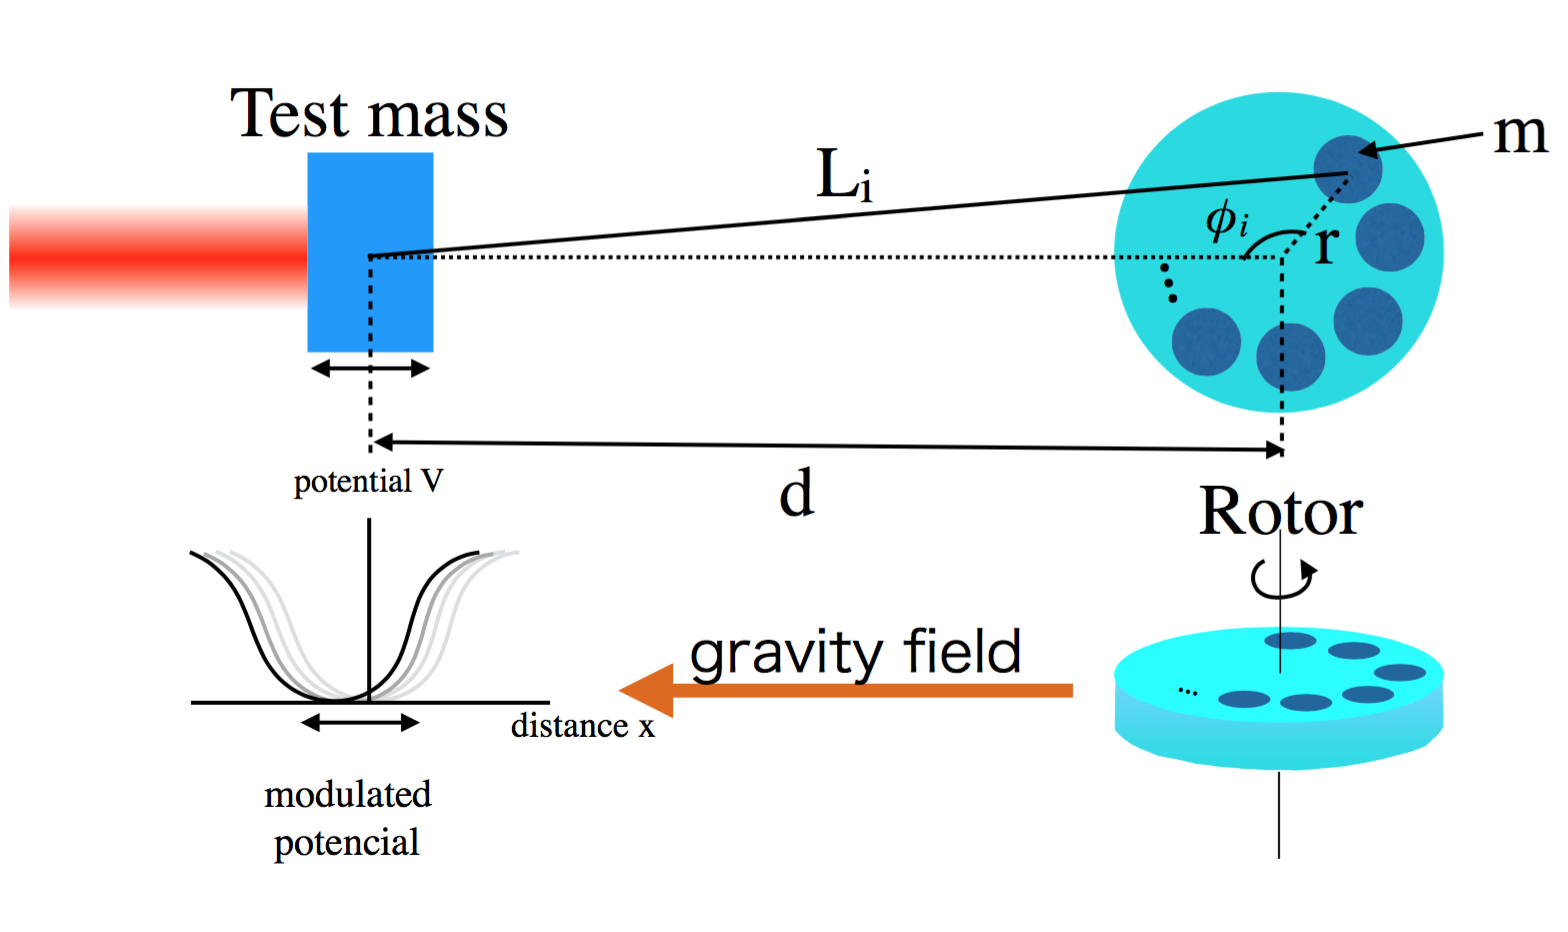
\includegraphics[width=12cm]{dim.eps}
\caption{Schematic view of gravity field calibrator. We placed the rotor at the displacement of $d$ away from test masses. Multipole mass generate the gravitational potential at the test mass position.}
\label{fig:dim}
\end{center}
\end{figure}

Distance between i-th mass and center of test mass is 
\begin{equation}
L_i=d \sqrt{1+\left( \frac{r}{d} \right)^2 -2\left( \frac{r}{d} \right) \cos{\phi_i} },
\end{equation}
where the angle of i-th mass is assumed as $\phi_i=\omega_{rot} t + 2\pi i/N$.
The gravity potential at the center of test mass can be described as
\begin{eqnarray}
V &=& \Sigma^N_{i=0} V_i \\
&=&-\frac{GMm}{d} \Sigma^N_{i=0} \Sigma^{\infty}_{n=0} \left( \frac{r}{d} \right)^n P_n\left(\cos{\left(\omega_{rot} t +\frac{2 \pi i}{N}\right)}\right),
\end{eqnarray}
where $P_n$ is Legendre polynomial. The equation of motion of test mass is 
\begin{equation}
Ma=\left| \frac{\partial V}{\partial{d}} \right| =\frac{GMm}{d^2}\Sigma^N_{i=0} \Sigma^{\infty}_{n=0}(n+1) \left( \frac{r}{d} \right)^n P_n\left(\cos{\left(\omega_{rot} t +\frac{2 \pi i}{N}\right)}\right),
\end{equation}
where $a$ is acceleration of test mass. We place the quadrupole and hexapole masses in same rotor as shown in Fig.~\ref{fig:hex}. We put the hole between each mass. The hole can increase the gravity gradient twice at the test massis. Therefore, we can describe the equation of motion as 
\begin{equation}
Ma=\left| \frac{\partial V}{\partial{d}} \right| =\frac{2GMm}{d^2}\Sigma^N_{i=0} \Sigma^{\infty}_{n=0}(n+1) \left( \frac{r}{d} \right)^n P_n\left(\cos{\left(\omega_{rot} t +\frac{2 \pi i}{N}\right)}\right),
\end{equation}
We will calculate the displacement of quadrupole and hexapole in the section ~\ref{Quad} 

\begin{figure}
\begin{center}
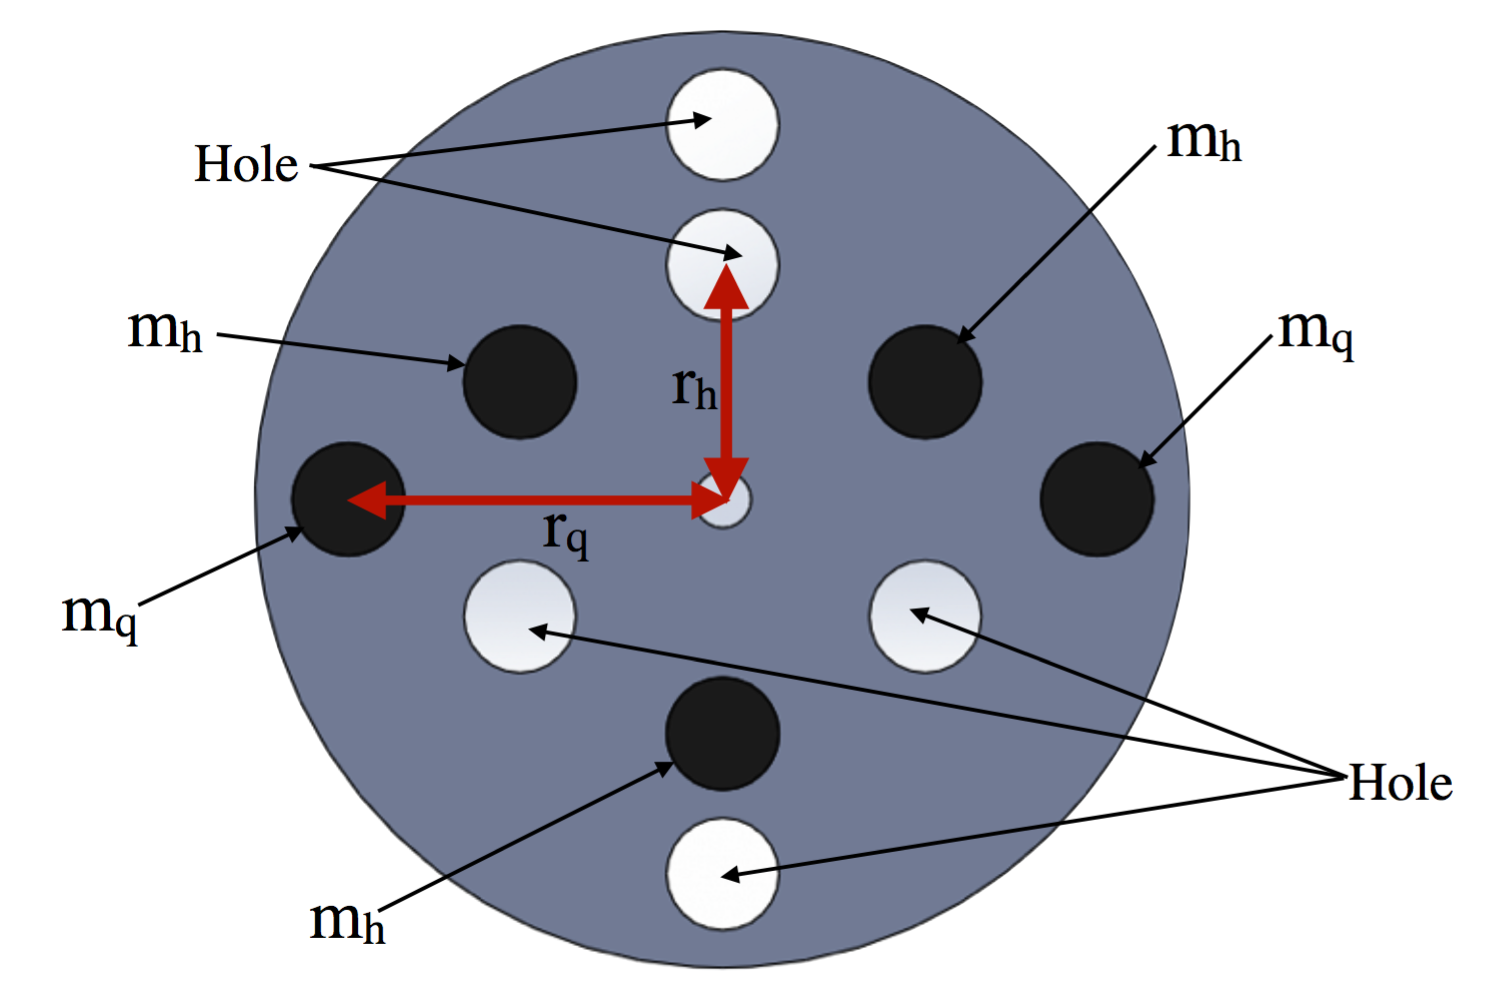
\includegraphics[width=12cm]{Hexapole.eps}
\caption{Configration of the rotor with quadrupole and haxapole mass distribution.$m_q$ and $m_h$ are mass of quadrupole and hexapole. $r_q$ and $r_h$ are radius of quadrupole and hexapole.}
\label{fig:hex}
\end{center}
\end{figure}

\subsection{Displacement of test mass(Quadrupole)} \label{Quad}
We calculate the displacement of the quadrupole mass distribution, which corresponds to $N=2$.
The mass and radius of quadrupole are assumed as $m_q$, $r_q$. 
The equation of motion of test mass is described as
\begin{equation}
Ma=\frac{2GMm_q}{d^2}\Sigma^{\infty}_{n=0}(n+1) \left( \frac{r_q}{d} \right)^n \left( P_n\left(\cos{\left(\omega_{rot} t \right)}\right) + P_n\left(\cos{\left(\omega_{rot} t +\pi \right)}\right) \right).
\end{equation} 
If we assume $r \ll d$, the displacement of the time-dependent lower harmonics can be written by 
\begin{equation}
x=\Sigma_{i=1}^{\infty}x_{n\mathrm{f}}\cos(n\omega_{rot} t)\sim x_{2\mathrm{f}}\cos(2\omega_{rot} t)=x_{2f}\cos{\omega t},
\end{equation}
where amplitude of 2-f rotation is
\begin{equation}
x_{2\mathrm{f}}=\frac{9}{4}\frac{GMm_{q}r_{q}^2}{d^4}s(\omega). \label{2f}
\end{equation}

\subsection{Displacement of test mass(Haxapole)} \label{Hexa}
We calculate the displacement of the hexapole mass distribution, which corresponds to $N=3$.
The mass and radius of hexapole are assumed as $m_h$, $r_h$. 
The equation of motion of test mass is described as
\begin{eqnarray}
Ma = \frac{2GMm_h}{d^2}\Sigma^{\infty}_{n=0}(n+1) \left( \frac{r_h}{d} \right)^n \\
\times \left( P_n\left(\cos{\left(\omega_{rot} t \right)}\right) + P_n\left(\cos{\left(\omega_{rot} t+\frac{2\pi}{3} \right)} \right) + P_n\left(\cos{\left(\omega_{rot} t \frac{4\pi}{3} \right) }\right) \right).
\end{eqnarray} 
If we assume $r \ll d$, the displacement of the time-dependent lower harmonics can be written by 
\begin{equation}
x=\Sigma_{i=1}^{\infty}x_{n\mathrm{f}}\cos(n\omega_{rot} t)\sim  x_{3\mathrm{f}}\cos(3\omega_{rot} t)=x_{3f}\cos{\omega t},
\end{equation}
where amplitude of 3-f is
\begin{equation}
 x_{3\mathrm{f}}=\frac{5}{3}\frac{GMm_{h}r_{h}^3}{d^5}s(\omega). \label{3f}
\end{equation}

\section{Absolute power calibration by using Gcal and Pcal}
In this section, we will discuss about absolute laser power calibration using interferometer. 
Figure~\ref{fig:IFO} shows the configuration of absolute laser power calibration by using the combination of photon calibrator and gravity field calibrator.
First, we modulate the mirror position using gravity field calibrator. We can measure the signal of $x_{2f}$ and $x_{3f}$ in the response o interferometer. Second, we send the interferometer signal to the excitation port of photon calibrator as a reference of feedback control. The photon calibrator cancel the displacement by gravity field calibrator. Third, we measure the absolute laser power at the detector of transmitter module and receiver module. The output signal of transmitter module, $V_{TxPD}$ and receiver module, $V_{RxPD}$ corresponding to displacement from gravity ffield should be modulated. By using Eq~(\ref{pcal}),(\ref{2f}), and (\ref{3f}), the modulated powers are
\begin{eqnarray}
 P_{2f}=\frac{9}{2} \frac{Gcm_{q}Mr_{q}^2}{d^4cos\theta}\frac{1}{1+\frac{M}{I}\vec{a}\cdot \vec{b}} \label{2f} \\
 P_{3f}= \frac{10}{3} \frac{Gcm_{h}Mr_{h}^3}{d^5cos\theta}\frac{1}{1+\frac{M}{I}\vec{a}\cdot \vec{b}} \label{3f}
\end{eqnarray}
Fourth, we demodulate the signal of transmitter module and receiver module using the encoder signal of gravity field calibrator.
The demodulated signals are 
\begin{eqnarray}
V_{2f}^{T}=\rho_{T}P_{2f} \\
V_{2f}^{R}=\rho_{R}P_{2f} \\
V_{3f}^{T}=\rho_{T}P_{3f} \\
V_{3f}^{R}=\rho_{R}P_{3f} 
\end{eqnarray} 
Therefore, we can estimate the distance using measured data. 
\begin{equation}
d=\frac{20}{27} \frac{V_{2f}^T}{V_{3f}^T}\frac{m_{h}}{m_{q}}\frac{r_{h}^{3}}{r_{q}^{2}}=\frac{20}{27} \frac{V_{2f}^R}{V_{3f}^R}\frac{m_{h}}{m_{q}}\frac{r_{h}^{3}}{r_{q}^{2}} \label{d}
\end{equation}
Using Eq (\ref{d}),(\ref{2f}) and (\ref{3f}), we can calibrate the absolute leaser power.
Finally, we insert the equatin (\ref{2f}) to the equation (\ref{pcal}):
\begin{eqnarray}
x&=&\frac{P_{2f} \cos{\theta}}{2c} s(\omega)\left(1+\frac{M}{I}\vec{a} \cdot \vec{b} \right) \\
 &=&\frac{9}{8}\frac{Gm_q M r_q^2}{d^4}s(\omega), \\
 &=&\frac{3^{14}}{5 \times 2^8} \frac{G m^5_q r_{q}^{14}}{m^4_h r_h^{12} \omega^2} \frac{V_{3f}^4}{V_{2f}^4}.
\end{eqnarray}
We estimate the  relative uncertainty of  displacement
\begin{eqnarray}
\left( \frac{\delta x}{x} \right)^2 &\sim& \left( \frac{\delta G}{G} \right)^2 +4\left( \frac{\delta \omega}{\omega} \right)^2+ 25\left( \frac{\delta m_q}{m_q} \right)^2 +16\left( \frac{\delta m_h}{m_h} \right)^2 \\
&+&16\left( \frac{\delta V_{f2}}{V_{f2}} \right)^2+16\left( \frac{\delta V_{f3}}{V_{f3}} \right)^2+ 196\left( \frac{\delta r_q}{r_q} \right)^2 +144\left( \frac{\delta r_h}{r_h} \right)^2 
\end{eqnarray}
\begin{figure}
\begin{center}
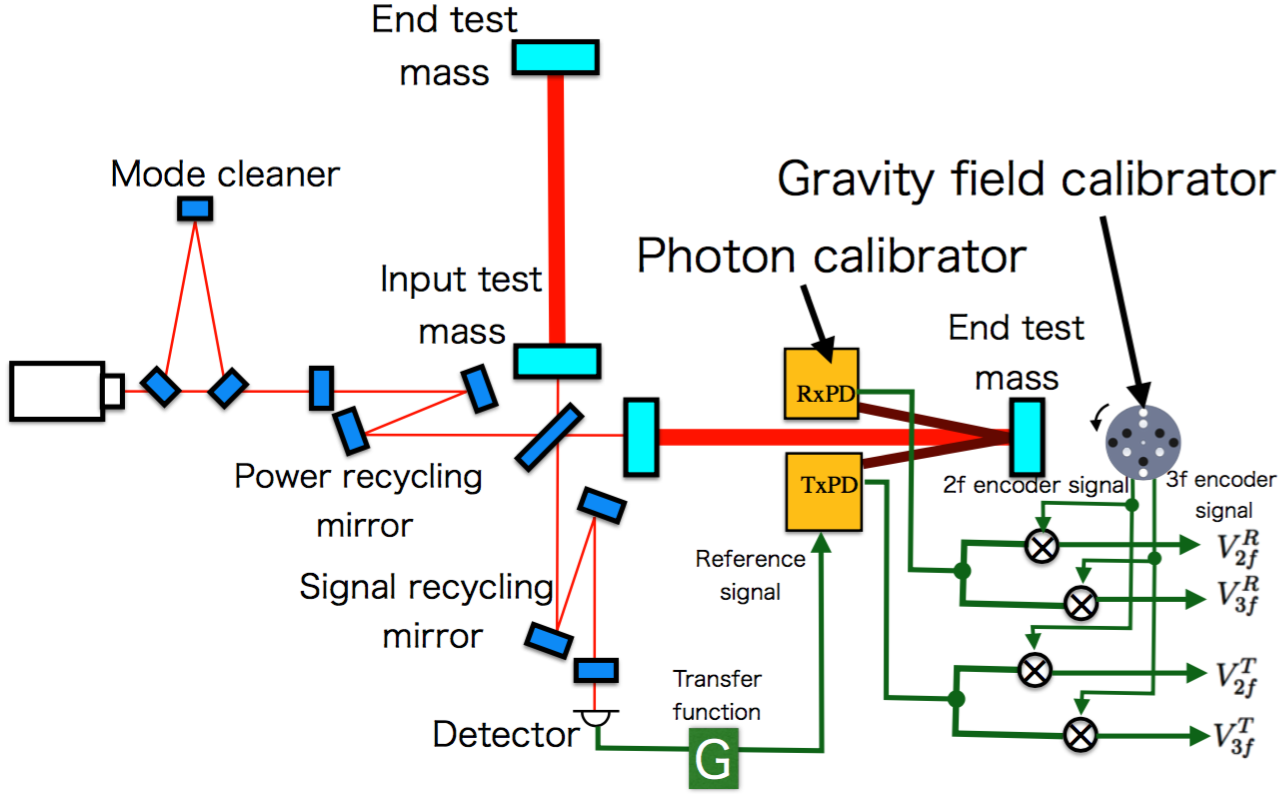
\includegraphics[width=12cm]{IFO.eps}
\caption{Test setup of the calibration of the laser power by rotating gravity field calibrator.}
\label{fig:IFO}
\end{center}
\end{figure}

\section{Estimation of uncertainty}
We estimate the uncertainty of laser power by assuming KAGRA. The assumed parameters are listed in Table XXX. We assumed the gaussian noise for each the parameters. We estimate the uncertainty of the laser power using Monte-Carlo simulation. The result is shown in Table XXXX. Table XXXX shows the uncertainty of  photon calibrator system based on LIGO system. By using Gcal system, we can reduce the uncertainty less than XXXX.
\begin{figure}
\begin{center}
\includegraphics[width=12cm]{peaks.eps}
\caption{}
\label{fig:peaks}
\end{center}
\end{figure}

\begin{table}
\begin{center}
\caption{\label{sus}The assumed parameters.}
\footnotesize
\begin{tabular}{ccc}
\br
$G$& Gravity constant&\\
$c$& speed of light[m/sec]&\\
$I$& Inertia[$\mathrm{kg m^2}$]&\\
$\theta$& Incident andgle[deg]&0.7\\
$M$& Mass of test mass[kg]&23\\
$m_q$&Mass of quadrupole[kg]&3.777\\
$m_h$&Mass of hexapole[kg]& 7.404\\
$r_q$&Radius of quadrupole[m]&0.130\\
$r_h$&Radius of hexapole[m]& 0.060\\
$d$&Distance[m]& 2.00\\
\br
\end{tabular}\\
\end{center}
\end{table}

\section{Discussion}
This method has an advantage of a direct comparison of the amplitude of injected power and gravity field. In previous study, we need to consider the uncertainty of the optical efficiency through the window and mirrors. This is because we put the working standard at the outside of the chamber. However, the compared gravity field can modulate the mirror directory.

We need to pay attention to the modulation effect of the intermediate mass because the gravity field act all the mass. 
伝達関数がキャンセルする利点こと。低い周波数だとIMの効果を入れないといけなく、伝達関数のズレがあること。
いつでも絶対キャリブレーションができること。
窓の効果率や積分球の効果を介さず計算できること。
r/dの数字によっては、1%の効果を考えるときにルジャンドル多項式の高次の効果を入れないといけない。有限要素法との比較。
ローターのパラメータのオプティマイズ。

\section{Summary}


\begin{verbatim}

\end{verbatim}



\end{document}

